\documentclass[12pt]{extarticle}
%Some packages I commonly use.
\usepackage[english]{babel}
\usepackage{graphicx}
\usepackage{framed}
\usepackage{url}
\usepackage[normalem]{ulem}
\usepackage{amsmath}
\usepackage{clrscode3e}
\usepackage{amsthm}
\usepackage{amssymb}
\usepackage{amsfonts}
\usepackage{enumerate}
\usepackage{indentfirst}
\usepackage[utf8]{inputenc}
\usepackage[top=1 in,bottom=1in, left=1 in, right=1 in]{geometry}
%A bunch of definitions that make my life easier
\newcommand{\matlab}{{\sc Matlab} }
\newcommand{\cvec}[1]{{\mathbf #1}}
\newcommand{\rvec}[1]{\vec{\mathbf #1}}
\newcommand{\ihat}{\hat{\textbf{\i}}}
\newcommand{\jhat}{\hat{\textbf{\j}}}
\newcommand{\khat}{\hat{\textbf{k}}}
\newcommand{\minor}{{\rm minor}}
\newcommand{\trace}{{\rm trace}}
\newcommand{\spn}{{\rm Span}}
\newcommand{\rem}{{\rm rem}}
\newcommand{\ran}{{\rm range}}
\newcommand{\range}{{\rm range}}
\newcommand{\mdiv}{{\rm div}}
\newcommand{\proj}{{\rm proj}}
\newcommand{\R}{\mathbb{R}}
\newcommand{\N}{\mathbb{N}}
\newcommand{\Q}{\mathbb{Q}}
\newcommand{\Z}{\mathbb{Z}}
\newcommand{\<}{\langle}
\renewcommand{\>}{\rangle}
\renewcommand{\emptyset}{\varnothing}
\newcommand{\attn}[1]{\textbf{#1}}
\theoremstyle{definition}
\newtheorem{theorem}{Theorem}
\newtheorem{corollary}{Corollary}
\newtheorem*{definition}{Definition}
\newtheorem*{example}{Example}
\newtheorem*{note}{Note}
\newtheorem{exercise}{Exercise}
\newcommand{\bproof}{\bigskip {\bf Proof. }}
\newcommand{\eproof}{\hfill\qedsymbol}
\newcommand{\Disp}{\displaystyle}
\newcommand{\qe}{\hfill\(\bigtriangledown\)}
\setlength{\columnseprule}{1 pt}
\title{F5:Gamma function}
\date{}
\author{Liangzhao Lin 40085480}
\begin{document}
\maketitle
\centerline {Repository: \url{https://github.com/linliangzhao/soen6011.git}}
\section{Changes from D1 to D2}
\begin{enumerate}[(1)]
\item Add the Repository Address to the top of my document.
\item Modify and update the Requirements analysis section.
\end{enumerate}

\section{Introduction of Gamma function }
\setlength{\parindent}{2em}
The gamma function$^{[1]}$ $\Gamma \left( x \right)$ is a transcendental function, which is a kind of function that the factorial function on real numbers and expands on complex numbers.
\newline
\indent
In the field of real numbers, the domain of this function is $x$ can be any real number except 0 and negative integer. The co-domain of this function is $(-{\infty},+{\infty}).$The image of the gamma function is shown in Figure 1.
\begin{figure}[ht]

\centering
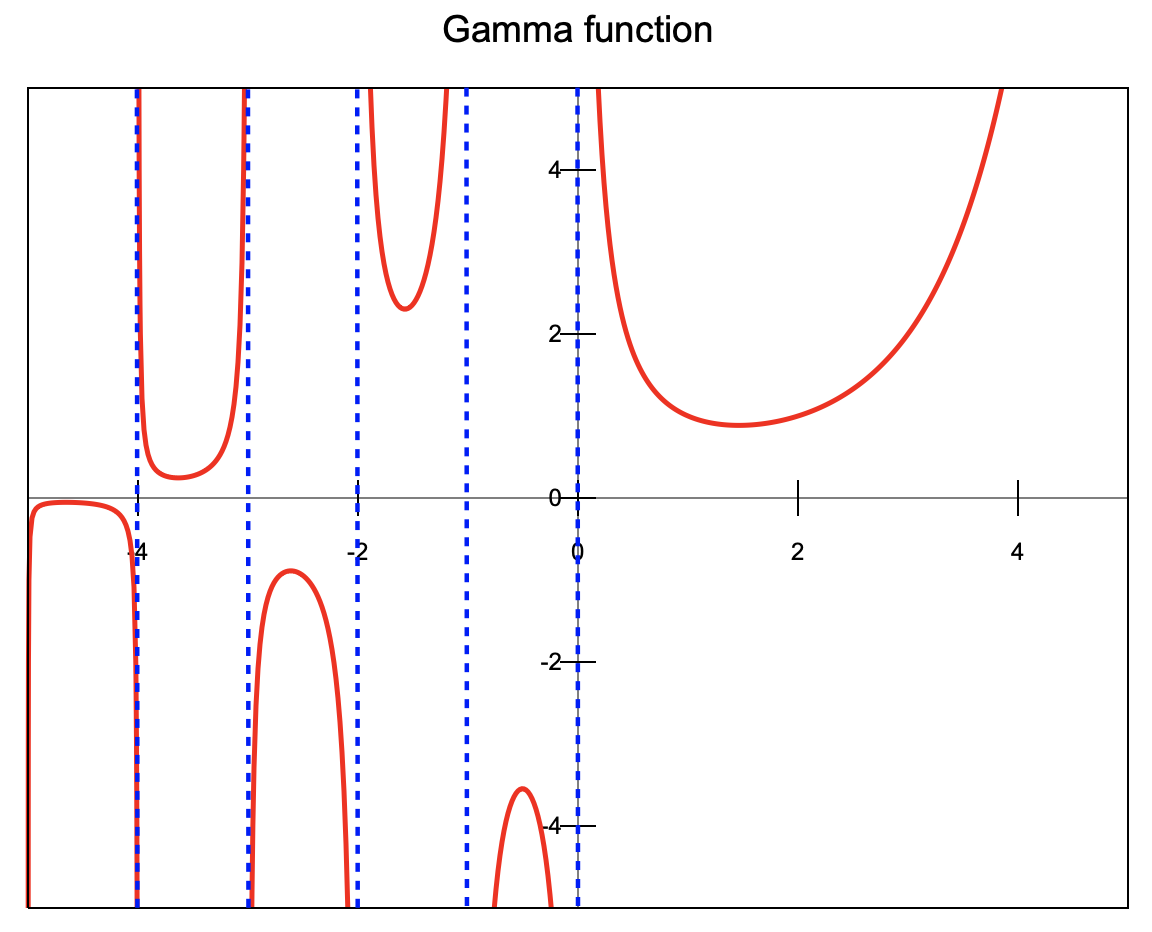
\includegraphics[scale=0.3]{gammafunction.png}
\caption{Gamma Function.  (Source: Google Images)}
\label{fig:label}
\end{figure}
\begin{enumerate}[(1)]

\item The gamma function is defined on the real number field as:$$\Gamma \left( x \right) = \int\limits_0^\infty {s^{x - 1} e^{ - s} ds}(x>0)$$
\item For a positive integer $x$, $\Gamma \left( x \right) = (x-1)!$
\item This function has recursive properties,  $\Gamma \left( x+1 \right) = x\Gamma\left( x \right) $
\end{enumerate}
\section{Requirements analysis}
\begin{enumerate}[\text{2.}1]
\item Functional requirement
\begin{enumerate}[\text{2.1.}1]
\item The user can enter any integer and finite decimal into the system.
\item The system can perform Gamma function calculation on the input $x$.
\item Display result. System shall display numbers to 6 significant digits after the decimal point, the function shall display the result in scientific notation.
\item When the input entered by the user is not a integer or finite decimal, the function shall return a message of error.
\end{enumerate}
\item Non-Functional requirement
\begin{enumerate}[\text{2.2.}1]
\item Portability. As long as the input is real number, all kinds of calculators can use this function directly. And the function can be implemented and used in both windows and MacOs operating systems.
\item Performance.The calculation range is integer and finite decimal. Fast calculations, all inputs can produce results in less than a second.
\item Reliability. The function result is high precision and the result is accurate.
\end{enumerate}

\end{enumerate}

\section {Algorithm selection}
\indent
Values of the gamma function can be computed numerically with high precision using Stirling's approximation algorithm or the Lanczos approximation algorithm. 
\begin{enumerate}[\text{3.}1]
\item Stirling's approximation algorithm
\newline
In mathematics, Stirling's approximation$^{[2]}$ is an approximation for factorials. The Stirling formula used to calculate the gamma function is:$$\Gamma \left( x+1 \right)\approx \sqrt{2\pi x}(\frac{x}{e})^{x}$$
The Figure2 illustrate the comparison of Stirling's approximation with the factorial.
\begin{figure}[ht]
\centering
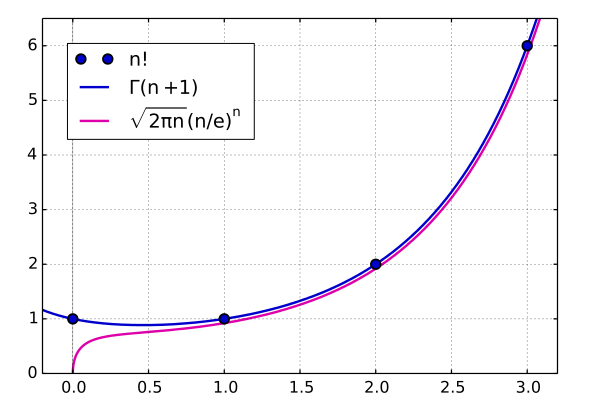
\includegraphics[scale=0.3]{figure2.png}
\caption{ \small Comparison of Stirling's approximation with the factorial.}
\end{figure}
\newline
\begin{enumerate}
\item[-]The advantage of Stirling's approximation algorithm is that when $x$ is large, their results are almost identical, moreover, even when $x$ is small, the result of the Stirling's approximation is also very accurate.
\newline
\item[-]The disadvantage is that this algorithm can not handle real numbers less than or equal to 0. 
\item[-]The pseudocode of Stirling's approximation algorithm is below:
\begin{codebox}
\Procname{$\proc{Stirling's approximation}(n)$}
\li $t$ = 1, $e$ = 2.718281828459, $pi$ = 3.14159265359
\li \For $i \gets 1$ \To $n$
\li     \Do
            $\id{t} \gets t*(n/e)$
\li         $i \gets i + 1$
        \End
\li $t = sqrt(2*pi*n)*t$
\li return $t$
\end{codebox}

\end{enumerate}
\item Lanczos approximation algorithm
\newline
The Lanczos approximation$^{[3]}$ is a method for computing the gamma function numerically,it is a practical alternative to the more popular Stirling's approximation for calculating the gamma function with fixed precision.
\begin{enumerate}

\item[-]The pseudocode of Lanczos approximation algorithm is below: 

\begin{codebox}
\Procname{$\proc{Lanczos approximation}(x)$}
\li $p=3.14159265359$
\li $t \gets (x-0.5)*log(x+4.5)-(4+4.5)$
\li $s \gets 1.0 + 76.18009173 / (x + 0) - 86.50532033 / (x + 1) + 24.01409822 / (x + 2)$ \\
$- 1.231739516 / (x + 3) + 0.00120858003 / (x + 4) - 0.00000536382 / (x + 5)$
\li $logGamma \gets t+log(s*sqrt(2*pi)$
\li $Gamma \gets exp(logGamma)$
\li return $Gamma$
\end{codebox}
\item[-]The advantage of Lanczos approximation algorithm is that this algorithm can calculate all the input in the gamma function domain.The precision of the calculation result can be adjusted and the result can be very accurate.
\item[-]The disadvantage is that the constant coefficient of each level in the formula is slightly more difficult to calculate, omitting the smallest coefficients does not result in a faster but slightly less accurate implementation.
\end{enumerate}
Overall, combined with the requirement analysis, Lanczos approximation algorithm is more suitable, it should be selected.
\end{enumerate}
\section{Quality attributes}
\setlength{\parindent}{2em}
In this section, I will introduce my efforts to implement the system to be correct, efficient, maintainable, robust, and usable.
\begin{enumerate}[(1)]
\item Correctness. For the user's legal input, the system can get a correct and high precision (accurate to 6 decimal places) results. This system is using the Lanczos algorithm.
each level constant coefficient of the Lanczos algorithm is accurate to 15 decimal places and the formula progresses to the 6th level series, making the result accurate.
\item Robustness. The system can only accept digital input. For invalid input, the system will not crash and can make error handling and feedback the causes. For example, if the input is not a valid rational number, the system can feedback “Input error, your input is not a number.". What's more, if the size of the input number exceeds the acceptable range of the double type, the system can feedback “Input error, the input is not a finite floating-point value."
\item Efficiency. This system can get results in one second for all inputs. For example, the formula $\Gamma \left( x \right) = \frac{\Gamma \left( x +1\right)}{x}$ is used in programming which need to use recursion, if the user's input is a negative number with large absolute values, it will cause too many recursive times, causing a long calculation time or even a stack overflow error.
\newline
In order to improve efficiency, I added a formal $\frac{\pi }{\Gamma \left( 1-x \right)\sin(\pi x)}$ to calculate the input of $x$ which is less than 2000, this can save system calculating time. Moreover, combined with the characteristics of the gamma function, the system directly outputs “Infinity" for inputs less than $-10^{8}$, as it does not need to step into the calculate function, so the system is highly efficient.
\item Usability. The user only needs to input the value of $x$ he wants to calculate, the system can return the value of $\Gamma \left( x \right)$, and for the illegal input, the system also returns the causes that the input is illegal, which can help the user to easily perform the gamma function.
\item Maintainable. The programming style of the project is using google programming style, every method and variable can understand its role by their name. What's more, the javadoc has been written for each method, so the workload required for maintenance is small. In addition, because the methods called for inputs in different intervals are different, it can be guided to methods that may have errors according to the input. For the output, different output statements will be executed according to the result in different intervals, so when finding the bug, the output statement can be used to trace the cause of the bug.
\end{enumerate}
\section{Brief introduction to Checkstyle}
\indent
I use Checkstyle tool to check the quality of my source code and keep the same programming style with my team.
\newline
\indent
Checkstyle is a static code analysis tool in software development$^{[4]}$ that checks if the Java source code matches the programming style. CheckStyle can automate the code specification checking process, the main content of the checking are Javadoc comments, name conventions, titles, line lengths, the use of imports and scope modifiers, interval between characters, etc. It helps us improve code readability in team projects, improve project quality, and make our projects easy to maintain. 
\newline
\indent
However, the disadvantage is that most of the functionality provided is for code specification checking, and does not provide as much enhancements to code quality and function like detecting flaws or possible flaws in source code.

\section {Brief introduction to Eclipse Debugger}
\indent
I use Eclipse Debugger tool to debug my project.
\newline
\indent
The Eclipse platform provides a built-in Java language debugger$^{[5]}$ that provides all the standard debugging features, including single stepping, setting breakpoints and values, checking variables and values, and the ability to suspend and resume threads, it can help programmers to perform error detection and diagnosis on the program.The Eclipse Debugger has multiple views, making the debugging process very convenient and intuitive.
\newline
\indent
However, the disadvantage that it does not have the smart step into function that the programmer can choose which method to enter when there are multiple method calls. In my opinion, I think this function can improve debugging efficiency.
\section{Unit testing with JUnit}
\indent
I use JUnit as the unit testing framework to test my function an use the results of apache.commons.math3 to compare the results of my gamma function. The test results are accurate to the eighth decimal place, and all test cases are successfully passed, which successfully meets the accuracy requirements of the display result in the requirement analysis.
\newline
\indent
My test case are $6$,$4.000001$,$32$,$-3.2$,$-0.00001$,$-42.232$,$-242.232$,$100.87$ and $-20.87$. These test cases can cover all input ranges that enable the gamma function of apache commons math3 to produce valid output without outputting $NaN$. The test results of these test cases can successfully pass the test, which proves that my function is consistent with the requirement.
\newline
\indent
In addition, I also use JUnit to test all the method of my gamma function and they all perform well.
\section{Reference}

\noindent[1] C. Lanczos, "A precision approximation of the gamma function," Journal of the Society for Industrial and Applied Mathematics, Series B: Numerical Analysis, vol. 1, (1), pp. 86-96, 1964.
\newline
[2] H. Robbins, "A remark on Stirling's formula," The American Mathematical Monthly, vol. 62, (1), pp. 26-29, 1955.
\newline
[3] P. J. Davis, "Leonhard Euler's integral: A historical profile of the Gamma function: In memoriam: Milton Abramowitz," The American Mathematical Monthly, vol. 66, (10), pp. 849-869, 1959. 
\newline
[4] O. Burn, "Checkstyle homepage," URL Http://checkstyle.Sourceforge.Net/.Last Accessed in March, vol. 14, 2005.
\newline
[5] J. K. Czyz and B. Jayaraman, "Declarative and visual debugging in eclipse," in Proceedings of the 2007 OOPSLA Workshop on Eclipse Technology eXchange, 2007, . 
\end{document}
